\documentclass[a4paper,14pt]{extarticle}
\usepackage{../../tex-shared/report-layout}

\renewcommand{\mylabnumber}{4}
\renewcommand{\mylabtitle}{Исследование процессов описания логики взаимодействия
                           информационных потоков при помощи методологии IDEF3 с
                           использованием CASE-средств}
\renewcommand{\mysubject}{Методы и средства проектирования информационных систем}
\renewcommand{\mylecturer}{Заикина Е.Н.}

\begin{document}
\begin{titlepage}
    
    \thispagestyle{empty}
    
    \begin{center}
        
        Министерство науки и Высшего образования Российской Федерации \\
        Севастопольский государственный университет \\
        Кафедра ИС
        
        \vfill

        Отчет \\
        по лабораторной работе №\mylabnumber \\
        \enquote{\mylabtitle} \\
        по дисциплине \\
        \enquote{\MakeTextUppercase{\mysubject}}

    \end{center}

    \vspace{1cm}

    \noindent\hspace{7.5cm} Выполнил студент группы ИС/б-17-2-о \\
    \null\hspace{7.5cm} Горбенко К. Н. \\
    \null\hspace{7.5cm} Проверил \\
    \null\hspace{7.5cm} \mylecturer

    \vfill

    \begin{center}
        Севастополь \\
        \the\year{}
    \end{center}

\end{titlepage}

\section{Цель работы}
\begin{itemize}
    \item осуществить функциональное моделирование процессов, ориентированное на
          потоки данных с помощью диаграмм логики взаимодействия информационных
          потоков в нотации IDEF3;
    \item осуществить выбор и применение инструментального средства описания
          логики взаимодействия информационных потоков (IDEF3 диаграммы).
\end{itemize}

\section{Задание на работу}
В соответствии с вариантом предметной области выполнить построение IDEF3
диаграммы при помощи CA ERwin Data Modeler Community Edition.

\section{Ход работы}
\begin{table}[H]
    \caption{Список действий и объектов, составляющих моделируемый процесс}
    \begin{tabular}{| c | c |}
        \hline
        № действия & Название действия \\ \hline
        1 & Работа со словарем \\ \hline
        2 & Регистрация \\ \hline
        3 & Создание группы словарей \\ \hline
        4 & Создание словаря \\ \hline
        5 & Получение упражнений \\ \hline
        6 & Создание группы словарей \\ \hline
        7 & Формирование списка предложений \\ \hline
        8 & Получение переводов для упражнений \\ \hline
        9 & Формирование правильных и неправильных ответов \\ \hline
        10 & Получение упражнений \\ \hline
    \end{tabular}
\end{table}

\begin{table}[H]
    \caption{Список действий с указанием предшествующих и последующих слбытий с указанием типа связи}
    \begin{tabular}{| p{3cm} | p{3cm} | p{3cm} | p{3cm} | p{3cm} |}
        \hline
        № или номера предшествующего действий & Тип связи & № действия & Тип связи & № или номера последующих действий \\ \hline
         & & 1 & & \\ \hline
         & & 2 & Временное предшествование & 3,4 \\ \hline
         3,4 & Объектный поток & 5 & & \\ \hline
         & & 6 & Объектный поток & 7 \\ \hline
         7 & Объектный поток & 8,9 & Объектный поток & 10 \\ \hline
         & & 10 & & \\ \hline
    \end{tabular}
\end{table}

\begin{table}[H]
    \caption{Список действий с указанием предшествующих и последующих событий с указанием установленных отношений}
    \begin{tabular}{| p{3cm} | p{3cm} | p{3cm} | p{3cm} | p{3cm} |}
        \hline
        № или номера предшествующего действий & Вид казуального отношения & № действия & Вид казуального отношения & № или номера последующих действий \\ \hline
        2 & Асинхронный \& & 3,4 & Асинхронный \& & 5 \\ \hline
        7 & Асинхронный \& & 8,9 & Синхронный \& & 10 \\ \hline
    \end{tabular}
\end{table}

На рисунках \ref{fig:context-diagram} - \ref{fig:exercise-receival-process}
представлены разработанные диаграммы в нотации \code{IDEF3}.

\begin{figure}[H]
    \centering
    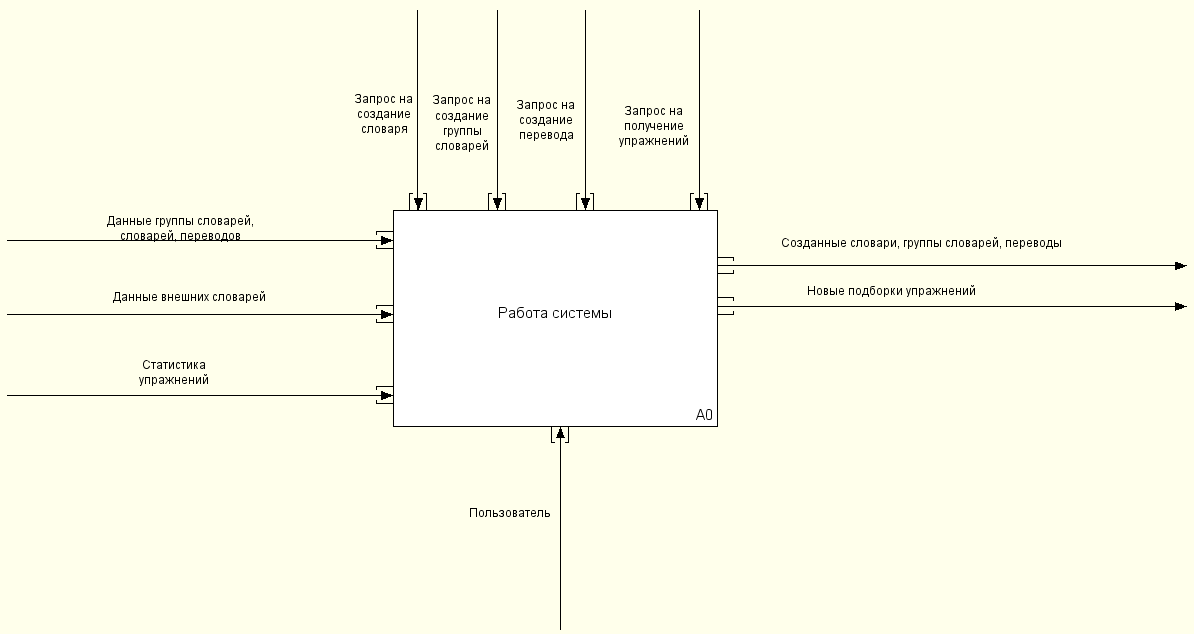
\includegraphics[width=\linewidth]{context-diagram}
    \caption{Диаграмма IDEF3 первого уровня}
    \label{fig:context-diagram}
\end{figure}

\begin{figure}[H]
    \centering
    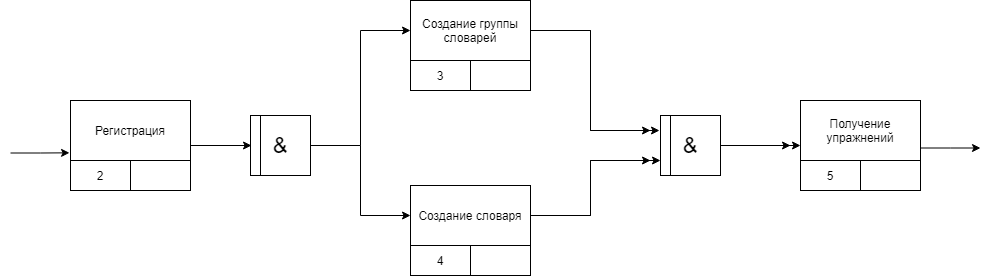
\includegraphics[width=\linewidth]{context-detailed}
    \caption{Диаграмма IDEF3 декомпозиции первого уровня}
    \label{fig:context-detailed}
\end{figure}

\begin{figure}[H]
    \centering
    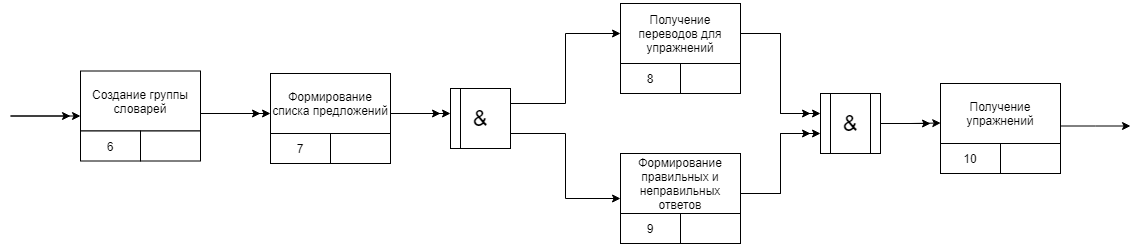
\includegraphics[width=\linewidth]{exercise-receival-process}
    \caption{Диаграмма IDEF3 декомпозиции действия 5}
    \label{fig:exercise-receival-process}
\end{figure}

\section*{Выводы}
В результате выполнения лабораторной работы было осуществлено функциональное
моделирование процессов, ориентированное на потоки данных с помощью диаграмм
логики взаимодействия информационных потоков в нотации IDEF3.

\end{document}